\documentclass[11pt]{article}

% -----------------------------------------------------------------------------
% Submission details: replace the bracketed fields before submission.
% -----------------------------------------------------------------------------
\newcommand{\studentname}{[Student name]}
\newcommand{\studentid}{[Student ID]}
\newcommand{\coursename}{[Course title and code]}
\newcommand{\instructorname}{[Instructor name]}
\newcommand{\submissiondate}{[Submission date]}

\usepackage[T1]{fontenc}
\usepackage[utf8]{inputenc}
\usepackage{lmodern}
\usepackage[margin=1in]{geometry}
\usepackage{microtype}
\usepackage{booktabs}
\usepackage{longtable}
\usepackage{array}
\usepackage{tabularx}
\usepackage{graphicx}
\usepackage{float}
\usepackage{amsmath,amssymb}
\usepackage{xcolor}
\usepackage{enumitem}
\usepackage{listings}
\usepackage{caption}
\usepackage{subcaption}
\usepackage{pdflscape}
\usepackage{hyperref}

\graphicspath{{figures/}}
\hypersetup{
  colorlinks=true,
  linkcolor=blue!55!black,
  urlcolor=blue!65!black,
  citecolor=blue!55!black,
  pdftitle={Political Violence During SSC and HSC Examinations},
  pdfauthor={\studentname}
}
\setlist{nosep}
\setlength{\parindent}{0pt}
\setlength{\parskip}{0.55em}
\renewcommand{\arraystretch}{1.15}

\definecolor{codebg}{RGB}{246,248,250}
\lstset{
  basicstyle=\ttfamily\small,
  backgroundcolor=\color{codebg},
  frame=single,
  rulecolor=\color{black!15},
  breaklines=true,
  columns=fullflexible,
  showstringspaces=false,
  language=Python
}

\newcommand{\sourceref}[1]{\textcolor{black!65}{\,[#1]}}
\newcommand{\pp}{percentage points}

\title{\textbf{Political Violence During SSC and HSC Examination Periods\\
and District-Level Examination Results in Bangladesh, 2011--2025}\\[0.5em]
\large A Two-Way Fixed-Effects Analysis}
\author{\studentname\\Student ID: \studentid\\\coursename\\Instructor: \instructorname}
\date{\submissiondate}

\begin{document}

\maketitle
\thispagestyle{empty}
\vfill
\begin{center}
\begin{minipage}{0.88\textwidth}
\small
\textbf{Submission note.} This report documents and interprets the complete workflow in the executed Jupyter notebook \texttt{political\_violence\_exam\_results\_twfe.ipynb}. It reports adjusted associations, not causal effects. The education workbook's original institutional source and the version of the UCDP extract from which the selected events were first taken were not recorded in the project metadata; this provenance limitation is disclosed throughout the report.
\end{minipage}
\end{center}
\vfill
\clearpage

\begin{abstract}
This study asks whether organized political violence occurring during Bangladesh's Secondary School Certificate (SSC) and Higher Secondary Certificate (HSC) examination periods is associated with district-level pass rates and A+ rates. The analysis combines a balanced district-year education panel for 64 districts from 2011 through 2025 with 227 selected events from the Uppsala Conflict Data Program Georeferenced Event Dataset (UCDP GED). Each examination window is defined as 50 inclusive calendar days beginning on the recorded examination start date. Event dates are represented either as exact days or closed uncertainty intervals. The primary exposure equals one when at least one located event falls definitely inside a district's examination window. Separate two-way fixed-effects regressions control for stable district differences and common year shocks; standard errors are clustered by district.

The usable samples contain 960 SSC district-years and 896 HSC district-years. Twenty-four SSC district-years and 32 HSC district-years are exposed under the primary definition. The estimated association with pass rates is approximately zero for both SSC (0.004 percentage points; 95\% CI $[-0.027, 0.035]$) and HSC ($-0.016$ percentage points; 95\% CI $[-0.046, 0.014]$). The SSC A+ coefficient is negative in the baseline model, whereas the HSC A+ coefficient is positive but uncertain. These A+ patterns change under reasonable robustness checks, especially when 2024 or influential districts are removed. The evidence therefore does not support a robust relationship between in-window violence and district pass rates. The A+ findings are exploratory and should not be interpreted causally.
\end{abstract}

\clearpage
\tableofcontents
\listoftables
\listoffigures
\clearpage

\section{Key Terms}

\begin{longtable}{p{0.24\textwidth}p{0.70\textwidth}}
\toprule
\textbf{Term} & \textbf{Meaning in this report} \\
\midrule
\endfirsthead
\toprule
\textbf{Term} & \textbf{Meaning in this report} \\
\midrule
\endhead
Association & A measured pattern in which two quantities vary together. An association does not by itself establish that one quantity caused the other. \\
A+ rate & The percentage of examinees in a district-year receiving an A+ result. \\
Binary exposure & A variable coded 1 when a district-year has at least one qualifying event and 0 otherwise. \\
Clustered standard error & An uncertainty estimate that permits observations from the same district to remain correlated across years. \\
Confidence interval (CI) & A range expressing statistical uncertainty around an estimate. The report uses 95\% intervals. \\
Definite overlap & A classification used when an event's full possible date interval lies inside the examination window. \\
District fixed effect & A control for all stable measured or unmeasured characteristics of a district. \\
Event intensity & The amount of measured violence, represented by event count or by the logarithm of one plus the reported deaths. \\
GED & The Georeferenced Event Dataset maintained by the Uppsala Conflict Data Program. \\
HSC & Higher Secondary Certificate examination. \\
Panel data & Repeated observations of the same districts over multiple years. \\
Pass rate & The percentage of examinees in a district-year recorded as passing. \\
Possible overlap & A classification used when any part of an event's possible date interval overlaps an examination window. \\
Political violence & In this report, the organized-violence events contained in the selected UCDP GED extract. This operational definition is narrower than every possible sociological meaning of political violence. \\
SSC & Secondary School Certificate examination. \\
Treated district-year & A district and year with at least one event satisfying the relevant exposure definition. \\
Two-way fixed effects (TWFE) & A regression design containing both district fixed effects and year fixed effects. \\
UCDP & Uppsala Conflict Data Program, the organization maintaining GED. \\
Year fixed effect & A control for shocks common to all districts in a particular year. \\
\bottomrule
\end{longtable}

\section{Background and Research Problem}

Examinations are institutionally timed events. Violence during an examination period could plausibly disrupt travel, attendance, preparation, concentration, or school administration. The available data make it possible to test whether district results are statistically different in years when a located organized-violence event occurs during the corresponding examination window. The outcome remains aggregated at district level, however, so the study cannot identify the experiences of individual students or schools.

The project links district-year SSC and HSC outcomes for Bangladesh's 64 districts to selected UCDP GED events. UCDP describes GED as an event-level dataset for organized violence with information about place, date, actors, and fatalities.\sourceref{UCDP GED codebook (2026/03), Sections 2--3} The standard academic introduction to GED is Sundberg and Melander (2013).\sourceref{Sundberg and Melander (2013), pp. 523--532}

The analytical question is deliberately narrow:

\begin{quote}
When a district experiences a qualifying political-violence event during an SSC or HSC examination window, is its district-level pass rate or A+ rate unusually high or low relative to both that district's usual outcome and the national pattern in that year?
\end{quote}

This question concerns an adjusted association. The design does not randomly assign violence, establish a counterfactual for each exposed district, or eliminate time-varying local confounding. Therefore, the term \emph{effect} is avoided when interpreting the coefficient substantively.

\section{Research Objectives and Hypotheses}

\subsection{Objectives}

The analysis has five objectives:

\begin{enumerate}
  \item validate the structure and timing fields of the two workbooks;
  \item construct transparent 50-day examination windows for SSC and HSC;
  \item aggregate located conflict events into district-year exposure measures;
  \item estimate district and year fixed-effects models for pass and A+ rates; and
  \item evaluate whether conclusions remain stable under alternative exposure and model choices.
\end{enumerate}

\subsection{Initial hypotheses}

\textbf{Primary null hypothesis (H0).} Political violence during an examination window has no association with the district pass rate after district and year fixed effects are included.

\textbf{Primary research hypothesis (H1).} Political violence during an examination window is associated with a lower district pass rate.

\textbf{Secondary hypothesis (H2).} Greater violence intensity, measured by event count or deaths, is associated with a lower district A+ rate.

These hypotheses were specified in the notebook before the results section. The pass-rate models are treated as primary. The A+ and intensity models are secondary and exploratory.

\section{Data and Provenance}

\subsection{Education data}

The education workbook contains one row for every district-year combination: 64 districts observed from 2011 through 2025, producing 960 rows. It includes SSC and HSC pass rates, A+ rates, examinee counts, education board, and examination start dates.\sourceref{Project README (2026/10), Data} The workbook's original institutional source is not recorded in the project README. Consequently, the numerical analysis is reproducible from the supplied workbook, but the education variables cannot presently be traced to a named original publication. This is a material provenance limitation, not a minor formatting issue.

HSC 2020 is excluded because the workbook does not contain a conventional examination date for that year and records an automatic-pass outcome rather than an ordinary examination result. The final model samples are therefore:

\begin{itemize}
  \item SSC: 960 observations, 64 districts, 15 years;
  \item HSC: 896 observations, 64 districts, 14 examination years.
\end{itemize}

\subsection{Conflict-event data}

The selected conflict workbook contains 227 event records. Each row includes a stable event identifier (\texttt{relid}), publication source, named location, location description, year, and UCDP's best estimate of deaths (\texttt{best}). The project identifies these records as selected UCDP GED events.\sourceref{Project README (2026/10), Data}

The original UCDP release from which the selected seven-column extract was created was not recorded. For the time-column update, every selected record was matched by exact \texttt{relid} to UCDP GED version 26.1. The matching script also required the event year and best death estimate to agree. All 227 records matched exactly once and passed these checks.\sourceref{Time-column method (2026/10), Source and matching}

\subsection{Where the event district came from}
\label{sec:district-provenance}

The event district was \textbf{not inferred inside the Jupyter notebook} and is not presented as a newly downloaded UCDP field. The notebook reads the pre-existing project-added \texttt{district} column from the dated conflict workbook with \texttt{pandas.read\_excel()}. It then excludes rows coded \texttt{Unknown} and groups qualifying events by \texttt{district}, \texttt{year}, and \texttt{exam}.

The district column had previously been populated by reading \texttt{where\_coordinates} and \texttt{where\_description}. A directly named district was used when present. District-headquarters cities were assigned to the district of the same name. Upazilas, towns, villages, camps, and neighbourhoods were mapped to their containing districts. Ambiguous cases were checked against the cited source article and contemporaneous reporting. Events with no recoverable subnational location were coded \texttt{Unknown}.\sourceref{District-mapping notes (2026/10), Method}

\begin{table}[H]
\centering
\caption{Provenance of event district assignments}
\label{tab:district-mapping}
\begin{tabular}{lr}
\toprule
\textbf{Assignment category} & \textbf{Events} \\
\midrule
Assigned directly from place name or description & 202 \\
Ambiguous or vague location checked individually & 12 \\
No recoverable district; coded \texttt{Unknown} & 13 \\
\midrule
Total & 227 \\
\bottomrule
\end{tabular}
\caption*{\footnotesize Source: District-mapping notes (2026/10), Summary. District names were standardized to the spelling used in the education workbook.}
\end{table}

Examples of administrative mapping include Savar, Mirpur, Gulshan, and Jatrabari to Dhaka; Ukhiya, Teknaf, and numbered Rohingya camps to Cox's Bazar; and Palash and Raipura to Narsingdi. Some events were less certain. The mapping documentation identifies Gopalpur as low confidence and several Shibganj, Kaliganj, and village-level cases as medium or medium-low confidence.\sourceref{District-mapping notes (2026/10), Method and researched events} These decisions can create geographic measurement error. The 13 \texttt{Unknown} events cannot contribute to district exposure and are excluded from the district-level models.

\subsection{How event time was populated}

The added \texttt{time} column comes from the official UCDP GED 26.1 fields \texttt{date\_start}, \texttt{date\_end}, and \texttt{date\_prec}; it does not use the publication date in \texttt{source\_article}.\sourceref{Time-column method (2026/10), Source and matching} Two representations are retained:

\begin{itemize}
  \item \texttt{YYYY-MM-DD} for an exact single-day event; and
  \item \texttt{YYYY-MM-DD/YYYY-MM-DD} for a closed interval from the earliest through latest possible date.
\end{itemize}

The dated workbook contains 204 exact dates and 23 date intervals. No time of day was inferred. UCDP treats the ordinary temporal unit as a local calendar day and uses date precision to represent uncertainty.\sourceref{UCDP GED codebook (2026/03), Sections 3 and 5.6; Time-column method (2026/10), Output format}

\section{Data Preparation and Exposure Construction}

\subsection{Validation}

The executed notebook stops with an assertion error if its core structural conditions fail. It verifies that the education panel contains 960 unique district-year rows, 64 districts, and 15 years; that the conflict table contains 227 unique event identifiers; that all time values are present; that every date interval ends on or after it begins; and that every event start year agrees with the recorded year.

\begin{table}[H]
\centering
\caption{Validation results from the executed notebook}
\label{tab:validation}
\begin{tabular}{lr}
\toprule
\textbf{Validation item} & \textbf{Value} \\
\midrule
Education district-years & 960 \\
Distinct districts & 64 \\
Years & 15 \\
Conflict events & 227 \\
Exact event dates & 204 \\
Event date ranges & 23 \\
Unlocated conflict events & 13 \\
\bottomrule
\end{tabular}
\end{table}

\subsection{Long-format education panel}

SSC and HSC variables are transformed from one wide district-year row into a long panel. A long-format row contains one district, one year, one examination, the appropriate board, pass rate, A+ rate, examinee count, and examination start date. This permits the same exposure-construction and regression functions to be applied separately to SSC and HSC without mixing their outcomes.

\subsection{Fifty-day examination windows}

The user-specified examination span is 50 days for both SSC and HSC. If an examination begins on date $S_{et}$ for examination $e$ in year $t$, the inclusive end date is

\begin{equation}
E_{et}=S_{et}+49\text{ days}.
\end{equation}

Adding 49 rather than 50 days is necessary because the start date counts as day one. The same national start and end dates apply to every district within a given examination-year in the supplied workbook; the notebook verifies one start-date value per examination-year.

For an event with earliest possible date $a_i$ and latest possible date $b_i$, the primary \emph{definite-overlap} rule is

\begin{equation}
Definite_{iet}=1\{a_i \geq S_{et}\;\text{and}\;b_i \leq E_{et}\}.
\end{equation}

The sensitivity \emph{possible-overlap} rule is

\begin{equation}
Possible_{iet}=1\{a_i \leq E_{et}\;\text{and}\;b_i \geq S_{et}\}.
\end{equation}

The first rule avoids inventing an event day when UCDP provides only an interval. The second asks whether any portion of that interval could fall in the examination period.

\subsection{District-year exposure variables}

Located events are joined to the national examination calendar by year, classified by the two overlap rules, and aggregated by district, year, and examination. The primary variable is

\begin{equation}
AnyViolence_{det}=1\{EventCount_{det}>0\}.
\end{equation}

Two intensity alternatives are also analyzed:

\begin{align}
EventCount_{det} &= \text{number of qualifying events},\\
LogDeaths_{det} &= \log(1+Deaths_{det}).
\end{align}

Adding one retains district-years with zero deaths, while the logarithm reduces the leverage of unusually deadly cells. Unexposed district-years receive zero for event count and deaths after the event aggregates are left-joined to the education panel.

\section{Statistical Method}

\subsection{Primary two-way fixed-effects model}

Separate models are estimated for each examination and outcome:

\begin{equation}
Y_{dt}=\beta V_{dt}+\alpha_d+\lambda_t+\varepsilon_{dt},
\label{eq:twfe}
\end{equation}

where $Y_{dt}$ is the district pass rate or A+ rate, $V_{dt}$ is the violence exposure, $\alpha_d$ is a district fixed effect, $\lambda_t$ is a year fixed effect, and $\varepsilon_{dt}$ is the remaining error. Because the outcome is measured in percent, $\beta$ is interpreted in percentage points.

District fixed effects compare each district with its own average, removing stable differences such as persistent geography or long-standing institutional conditions. Year fixed effects remove national changes shared by all districts in a given year, such as a nationally easier examination. Identification therefore comes from within-district changes in exposure after common yearly patterns are removed.

\subsection{Estimation and uncertainty}

The notebook creates indicator variables for all but one district and all but one year, includes an intercept and exposure variable, and solves the ordinary least-squares problem with \texttt{numpy.linalg.lstsq}. It calculates a district-clustered sandwich covariance matrix. In compact form,

\begin{equation}
\widehat{Var}(\hat\beta)=c(X'X)^{-1}
\left(\sum_{g=1}^{G}X_g'\hat u_g\hat u_g'X_g\right)(X'X)^{-1},
\end{equation}

where $g$ indexes districts, $G$ is the number of district clusters, and $c$ is the finite-sample correction implemented in the notebook. The correction is

\begin{equation}
c=\frac{G}{G-1}\frac{n-1}{n-r},
\end{equation}

with $n$ observations and design-matrix rank $r$. Confidence intervals use the large-sample normal critical value 1.96, and two-sided p-values use the standard normal distribution. With 64 clusters in the main models this is a conventional approximation, but a small-cluster correction based on a $t$ distribution or wild-cluster bootstrap was not implemented.

\subsection{Robustness specifications}

Five specifications are compared:

\begin{enumerate}
  \item \textbf{Baseline:} definite in-window binary exposure with district and year fixed effects.
  \item \textbf{Possible overlap:} any partial overlap of an uncertain date range counts as exposure.
  \item \textbf{Exclude 2024:} tests sensitivity to the year dominating HSC exposure.
  \item \textbf{Exclude Dhaka and Cox's Bazar:} tests sensitivity to two high-event districts.
  \item \textbf{Board-by-year controls:} replaces national year indicators with education-board-by-year indicators, allowing annual shocks to differ across boards.
\end{enumerate}

The notebook does not adjust p-values for the number of secondary and robustness models. Accordingly, isolated small p-values should not be treated as confirmatory evidence without preregistration or replication.

\section{Descriptive Results}

\subsection{Outcome trends}

Figure~\ref{fig:pass-trends} plots the unweighted mean district pass rate by year. SSC and HSC rates both vary substantially over time. HSC 2020 is absent because no conventional examination was held in the supplied data. The very high 2021 averages and the later decline reinforce the need for year controls: raw comparisons between exposed and unexposed years could otherwise confuse violence exposure with nationwide changes.

\begin{figure}[H]
\centering
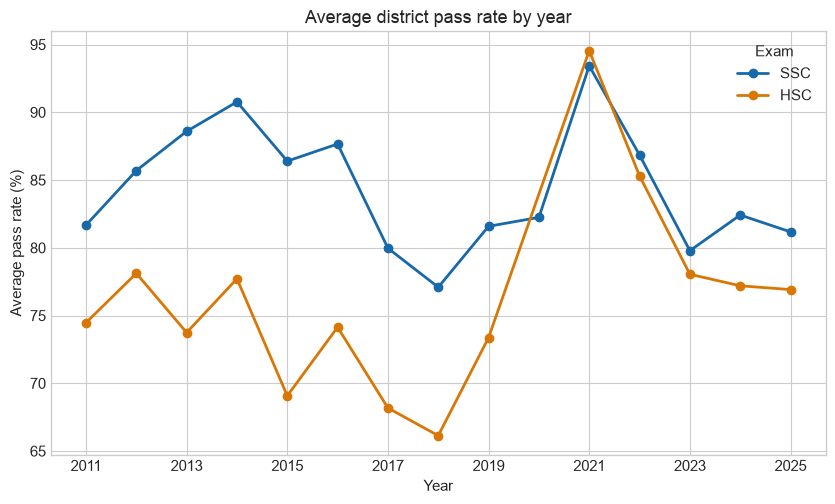
\includegraphics[width=0.92\textwidth]{average_pass_rate_by_year.png}
\caption{Average district pass rate by year and examination}
\label{fig:pass-trends}
\caption*{\footnotesize Source: Author's calculations from the supplied education workbook. Averages are unweighted across districts.}
\end{figure}

\subsection{Availability and concentration of exposure}

\begin{table}[H]
\centering
\caption{Primary in-window violence exposure}
\label{tab:window-summary}
\resizebox{\textwidth}{!}{%
\begin{tabular}{lrrrrr}
\toprule
\textbf{Exam} & \textbf{Located events} & \textbf{Deaths} & \textbf{Treated district-years} & \textbf{Treated districts} & \textbf{Usable district-years} \\
\midrule
SSC & 32 & 42 & 24 & 16 & 960 \\
HSC & 59 & 168 & 32 & 27 & 896 \\
\bottomrule
\end{tabular}}
\caption*{\footnotesize Located events are events assigned to a district whose full possible date interval lies inside the 50-day window. Deaths use UCDP's \texttt{best} estimate.}
\end{table}

Only 2.5\% of SSC district-years (24 of 960) and approximately 3.6\% of HSC district-years (32 of 896) are treated. Figure~\ref{fig:exposure-year} shows that exposure is highly concentrated in particular years. For HSC, 2024 alone contributes 47 of 59 definite in-window events and 146 of 168 deaths. SSC exposure is more dispersed but 2013 contributes 13 of 32 events and 20 of 42 deaths.

\begin{figure}[H]
\centering
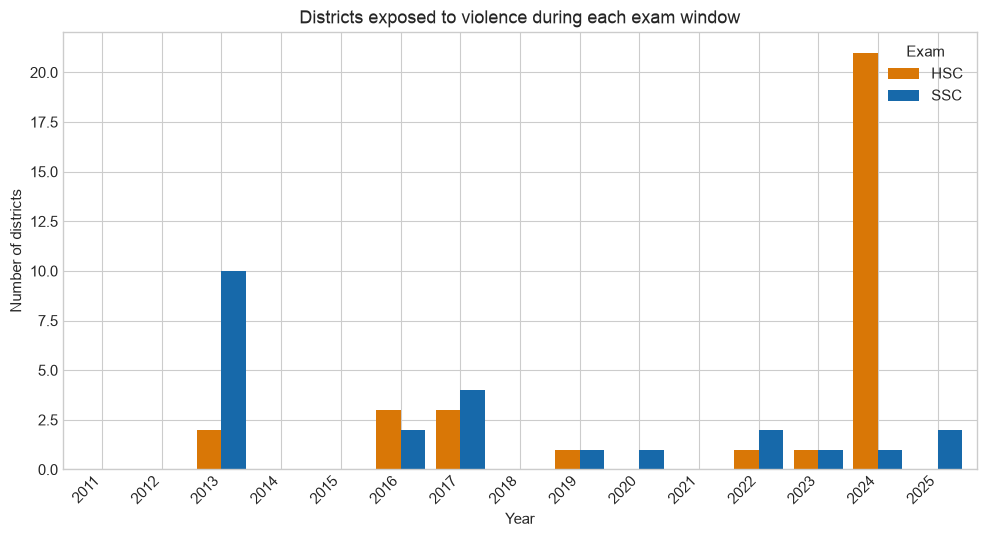
\includegraphics[width=0.94\textwidth]{districts_exposed_by_year.png}
\caption{Number of exposed districts by year and examination}
\label{fig:exposure-year}
\caption*{\footnotesize Exposure means at least one located event definitely inside the 50-day examination window.}
\end{figure}

\begin{table}[H]
\centering
\caption{Definite in-window events and deaths by examination-year}
\label{tab:concentration}
\begin{tabular}{lrr@{\qquad}lrr}
\toprule
\textbf{Exam-year} & \textbf{Events} & \textbf{Deaths} & \textbf{Exam-year} & \textbf{Events} & \textbf{Deaths} \\
\midrule
HSC 2013 & 3 & 9 & SSC 2013 & 13 & 20 \\
HSC 2016 & 3 & 3 & SSC 2016 & 2 & 2 \\
HSC 2017 & 3 & 6 & SSC 2017 & 5 & 8 \\
HSC 2019 & 1 & 2 & SSC 2019 & 1 & 0 \\
HSC 2022 & 1 & 1 & SSC 2020 & 1 & 1 \\
HSC 2023 & 1 & 1 & SSC 2022 & 4 & 5 \\
HSC 2024 & 47 & 146 & SSC 2023 & 1 & 1 \\
 & & & SSC 2024 & 3 & 3 \\
 & & & SSC 2025 & 2 & 2 \\
\bottomrule
\end{tabular}
\end{table}

This concentration matters for interpretation. A fixed-effects coefficient may be mathematically estimable while still depending strongly on a small number of district-years or one unusual national period.

\section{Main Two-Way Fixed-Effects Results}

\begin{table}[H]
\centering
\caption{Baseline TWFE estimates for any definite in-window event}
\label{tab:main-results}
\resizebox{\textwidth}{!}{%
\begin{tabular}{llrrrrrr}
\toprule
\textbf{Exam} & \textbf{Outcome} & \textbf{Estimate} & \textbf{Clustered SE} & \textbf{95\% CI} & \textbf{$p$} & \textbf{$N$} & \textbf{Treated cells} \\
\midrule
SSC & Pass rate & 0.004 & 0.016 & $[-0.027,\;0.035]$ & 0.806 & 960 & 24 \\
SSC & A+ rate & $-0.246$ & 0.095 & $[-0.432,\;-0.059]$ & 0.010 & 960 & 24 \\
HSC & Pass rate & $-0.016$ & 0.015 & $[-0.046,\;0.014]$ & 0.300 & 896 & 32 \\
HSC & A+ rate & 0.345 & 0.198 & $[-0.043,\;0.734]$ & 0.081 & 896 & 32 \\
\bottomrule
\end{tabular}}
\caption*{\footnotesize Estimates are percentage-point associations. All models include district and year fixed effects. Standard errors are clustered by district.}
\end{table}

The SSC pass-rate estimate is 0.004 percentage points, which is substantively negligible and statistically imprecise around zero. The HSC pass-rate estimate is also small at $-0.016$ percentage points. Both confidence intervals cross zero. Thus the primary models provide no evidence of a robust negative pass-rate association.

The SSC A+ estimate is $-0.246$ percentage points and its baseline confidence interval excludes zero. The HSC A+ estimate is 0.345 percentage points, but its interval includes zero and its sign is opposite to the secondary hypothesis. These A+ coefficients require careful sensitivity analysis because they are secondary outcomes and exposure is sparse.

\begin{figure}[H]
\centering
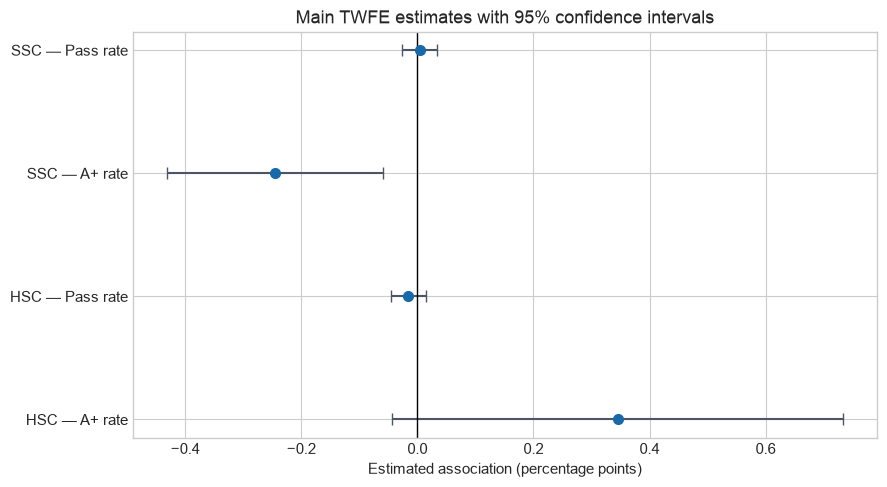
\includegraphics[width=0.88\textwidth]{main_twfe_estimates.png}
\caption{Main TWFE coefficients and 95\% confidence intervals}
\label{fig:main-coefficients}
\caption*{\footnotesize Points are estimated percentage-point associations. Horizontal bars are 95\% normal-approximation confidence intervals.}
\end{figure}

\section{Alternative Violence-Intensity Models}

{\small
\setlength{\tabcolsep}{4pt}
\begin{longtable}{lllrrrr}
\caption{Alternative violence measures}\label{tab:intensity}\\
\toprule
\textbf{Exam} & \textbf{Outcome} & \textbf{Exposure} & \textbf{Estimate} & \textbf{SE} & \textbf{95\% CI} & \textbf{$p$} \\
\midrule
\endfirsthead
\toprule
\textbf{Exam} & \textbf{Outcome} & \textbf{Exposure} & \textbf{Estimate} & \textbf{SE} & \textbf{95\% CI} & \textbf{$p$} \\
\midrule
\endhead
SSC & Pass rate & Any event & 0.004 & 0.016 & $[-0.027,0.035]$ & 0.806 \\
SSC & Pass rate & Event count & 0.003 & 0.008 & $[-0.013,0.019]$ & 0.718 \\
SSC & Pass rate & $\log(1+\text{deaths})$ & 0.011 & 0.013 & $[-0.014,0.036]$ & 0.384 \\
SSC & A+ rate & Any event & $-0.246$ & 0.095 & $[-0.432,-0.059]$ & 0.010 \\
SSC & A+ rate & Event count & $-0.213$ & 0.061 & $[-0.333,-0.094]$ & $<0.001$ \\
SSC & A+ rate & $\log(1+\text{deaths})$ & $-0.363$ & 0.089 & $[-0.537,-0.189]$ & $<0.001$ \\
HSC & Pass rate & Any event & $-0.016$ & 0.015 & $[-0.046,0.014]$ & 0.300 \\
HSC & Pass rate & Event count & 0.000 & 0.002 & $[-0.003,0.004]$ & 0.801 \\
HSC & Pass rate & $\log(1+\text{deaths})$ & $-0.007$ & 0.008 & $[-0.023,0.008]$ & 0.354 \\
HSC & A+ rate & Any event & 0.345 & 0.198 & $[-0.043,0.734]$ & 0.081 \\
HSC & A+ rate & Event count & 0.164 & 0.029 & $[0.107,0.221]$ & $<0.001$ \\
HSC & A+ rate & $\log(1+\text{deaths})$ & 0.324 & 0.117 & $[0.095,0.554]$ & 0.006 \\
\bottomrule
\end{longtable}
}

The pass-rate conclusion is stable: event count and logged deaths remain close to zero for both examinations. The A+ intensity coefficients are negative for SSC but positive for HSC. Opposite signs across examinations do not support a single general relationship between violence intensity and high achievement. The positive HSC estimates are especially vulnerable to the concentration of 47 events and 146 deaths in the 2024 window.

The scales also differ across rows. The event-count coefficient is the estimated outcome difference associated with one additional event, whereas the logged-deaths coefficient corresponds to a one-unit increase in $\log(1+\text{deaths})$. These are not directly comparable effect sizes.

\section{Robustness Analysis}

\begin{landscape}
{\small
\setlength{\tabcolsep}{5pt}
\begin{longtable}{lllrrrr}
\caption{Robustness specifications}\label{tab:robustness}\\
\toprule
\textbf{Exam} & \textbf{Outcome} & \textbf{Specification} & \textbf{Estimate} & \textbf{SE} & \textbf{95\% CI} & \textbf{$p$} \\
\midrule
\endfirsthead
\toprule
\textbf{Exam} & \textbf{Outcome} & \textbf{Specification} & \textbf{Estimate} & \textbf{SE} & \textbf{95\% CI} & \textbf{$p$} \\
\midrule
\endhead
SSC & Pass & Baseline & 0.004 & 0.016 & $[-0.027,0.035]$ & 0.806 \\
SSC & Pass & Possible overlap & 0.004 & 0.016 & $[-0.027,0.035]$ & 0.806 \\
SSC & Pass & Exclude 2024 & 0.003 & 0.016 & $[-0.028,0.035]$ & 0.838 \\
SSC & Pass & Exclude Dhaka/Cox's Bazar & 0.013 & 0.019 & $[-0.023,0.050]$ & 0.472 \\
SSC & Pass & Board-by-year controls & $-0.007$ & 0.010 & $[-0.026,0.012]$ & 0.469 \\
SSC & A+ & Baseline & $-0.246$ & 0.095 & $[-0.432,-0.059]$ & 0.010 \\
SSC & A+ & Possible overlap & $-0.246$ & 0.095 & $[-0.432,-0.059]$ & 0.010 \\
SSC & A+ & Exclude 2024 & $-0.230$ & 0.095 & $[-0.416,-0.044]$ & 0.015 \\
SSC & A+ & Exclude Dhaka/Cox's Bazar & $-0.169$ & 0.105 & $[-0.374,0.036]$ & 0.106 \\
SSC & A+ & Board-by-year controls & $-0.275$ & 0.154 & $[-0.578,0.027]$ & 0.075 \\
HSC & Pass & Baseline & $-0.016$ & 0.015 & $[-0.046,0.014]$ & 0.300 \\
HSC & Pass & Possible overlap & $-0.016$ & 0.015 & $[-0.046,0.014]$ & 0.300 \\
HSC & Pass & Exclude 2024 & $-0.059$ & 0.031 & $[-0.119,0.002]$ & 0.057 \\
HSC & Pass & Exclude Dhaka/Cox's Bazar & $-0.017$ & 0.018 & $[-0.051,0.018]$ & 0.340 \\
HSC & Pass & Board-by-year controls & 0.001 & 0.008 & $[-0.014,0.016]$ & 0.946 \\
HSC & A+ & Baseline & 0.345 & 0.198 & $[-0.043,0.734]$ & 0.081 \\
HSC & A+ & Possible overlap & 0.345 & 0.198 & $[-0.043,0.734]$ & 0.081 \\
HSC & A+ & Exclude 2024 & $-0.196$ & 0.235 & $[-0.657,0.265]$ & 0.404 \\
HSC & A+ & Exclude Dhaka/Cox's Bazar & 0.436 & 0.216 & $[0.014,0.858]$ & 0.043 \\
HSC & A+ & Board-by-year controls & 0.348 & 0.228 & $[-0.100,0.795]$ & 0.128 \\
\bottomrule
\end{longtable}
}
\end{landscape}

\begin{figure}[H]
\centering
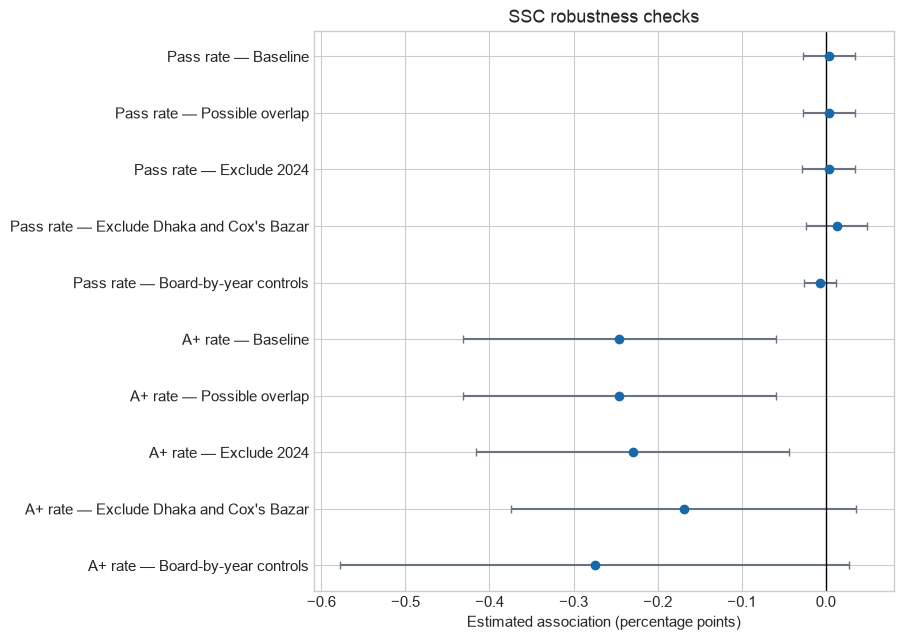
\includegraphics[width=0.96\textwidth]{ssc_robustness.png}
\caption{SSC robustness coefficients with 95\% confidence intervals}
\label{fig:ssc-robustness}
\end{figure}

\begin{figure}[H]
\centering
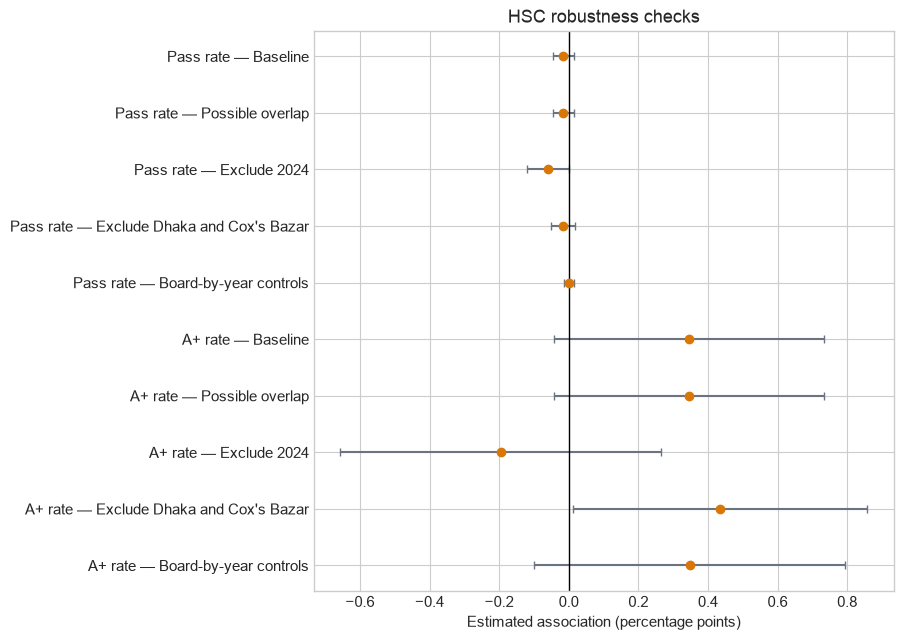
\includegraphics[width=0.96\textwidth]{hsc_robustness.png}
\caption{HSC robustness coefficients with 95\% confidence intervals}
\label{fig:hsc-robustness}
\end{figure}

The SSC and HSC pass-rate estimates remain small in most specifications. Excluding 2024 makes the HSC pass coefficient more negative ($-0.059$), but its 95\% interval still narrowly includes zero. Board-by-year controls move it back to approximately zero. This pattern does not establish a stable negative association.

The SSC A+ coefficient remains negative when 2024 is removed, but its interval crosses zero after excluding Dhaka and Cox's Bazar and after using board-by-year controls. The HSC A+ estimate changes from 0.345 in the baseline to $-0.196$ when 2024 is excluded. This sign reversal is direct evidence that the positive baseline pattern depends strongly on the unusual 2024 exposure concentration. Removing Dhaka and Cox's Bazar produces a positive estimate whose interval excludes zero, but this isolated result is not stable across the other specifications.

The definite- and possible-overlap models are identical in this sample. This indicates that none of the uncertain date intervals changes district-year treatment status under the broader overlap rule for these examination windows.

\section{Findings and Hypothesis Decisions}

\subsection{Primary finding: pass rates}

The most stable result is a near-zero relationship between in-window violence and district pass rates. Both baseline pass-rate confidence intervals cross zero; event-count and death-intensity alternatives remain near zero; and robustness estimates do not reveal a consistent negative pattern. H0 therefore cannot be rejected consistently for pass rates, and H1 is not supported by the analyzed data.

Failing to reject H0 is not proof that violence has no educational consequences. The study may have limited power because treatment is rare, outcomes are aggregated, exposure is geographically imperfect, and disruption may operate outside the chosen 50-day period. The defensible claim is narrower: this design and dataset do not reveal a robust district pass-rate association.

\subsection{Secondary finding: A+ rates}

SSC A+ estimates are negative in the baseline and intensity models, while HSC estimates are positive in the baseline intensity models. The patterns are neither directionally consistent across examinations nor stable across sensitivity checks. H2 therefore receives mixed and unstable support rather than confirmation. These results should motivate additional data collection and theory development, not a conclusion that violence reliably raises or lowers high achievement.

\subsection{Sociological interpretation}

District pass rates may be institutionally buffered by examination rescheduling, administrative responses, grading practices, or aggregation across many schools, while more localized disruptions remain invisible in district averages. These mechanisms were not measured in the supplied data, so they are possible interpretations rather than tested explanations. Similarly, a district-level event may affect students in adjacent districts through fear, transport disruption, media exposure, or school closure. The model treats districts as separate exposure units and cannot estimate these spillovers.

\section{Limitations}

\begin{enumerate}
  \item \textbf{No causal identification.} District and year fixed effects remove stable district differences and common yearly shocks, but they do not remove unobserved district conditions that change over time. Political competition, strikes, local economic shocks, school closures, or administrative responses could influence both violence and results.

  \item \textbf{Sparse treatment.} Only 24 SSC and 32 HSC district-years are treated. Sparse exposure increases uncertainty and makes coefficients sensitive to individual observations.

  \item \textbf{Temporal concentration.} Forty-seven of 59 HSC events occur in 2024. The HSC A+ coefficient reverses sign when that year is removed.

  \item \textbf{District assignment uncertainty.} The notebook accepts a project-added district column. Twelve ambiguous cases were researched individually, at least one is documented as low confidence, and 13 events remain unlocated. Misclassification can alter district-year exposure.

  \item \textbf{Unlocated events.} Events coded \texttt{Unknown} are excluded. If they occurred in otherwise untreated districts during examination windows, exposure is understated.

  \item \textbf{Selected definition of political violence.} The dataset includes selected UCDP organized-violence events. It may omit nonlethal intimidation, threats, strikes, blockades, school attacks, or other disruptions relevant to education.

  \item \textbf{Outcome aggregation.} District averages can conceal heterogeneous effects by school, gender, class, disability, rurality, or household socioeconomic position.

  \item \textbf{Window choice.} The 50-day span was specified by the user. It may exclude violence immediately before examinations, when preparation is affected, or after the nominal end date if examinations were delayed.

  \item \textbf{Spillovers.} Violence in one district may affect neighboring districts. This violates the simple assumption that one district's exposure is unrelated to another district's outcome.

  \item \textbf{Provenance gaps.} The original education source and original UCDP extract version were not recorded. Event dates are traceable to GED 26.1, but the selected event extract may have originated from another release. UCDP notes that records can be revised between releases.\sourceref{UCDP GED codebook (2026/03), Section 3}

  \item \textbf{Inference and multiple analysis choices.} The notebook uses a normal approximation with cluster-robust standard errors and does not apply a multiple-testing adjustment. Secondary p-values should therefore be read cautiously.
\end{enumerate}

\section{Recommendations for a Stronger Follow-up Study}

\begin{enumerate}
  \item Record and cite the original source of every education variable and the exact UCDP release used to select events.
  \item Audit medium- and low-confidence district assignments using archived local reporting or official administrative records.
  \item Add school- or upazila-level outcomes so local disruption is not averaged across an entire district.
  \item Measure school closures, strikes, transport shutdowns, examination postponements, and violence in the weeks before each examination.
  \item Pre-register the exposure window, primary outcome, and principal robustness checks before re-estimating the model.
  \item Examine spatial spillovers by measuring exposure in adjacent districts and distance to events.
  \item Use event-study or matched designs only after testing whether their identifying assumptions and pre-treatment information are adequate.
  \item Consider randomization inference or wild-cluster bootstrap methods for uncertainty, particularly in specifications with few treated clusters.
\end{enumerate}

\section{Conclusion}

The analysis is feasible after adding event dates and using the project-assigned event districts. The main pass-rate result is straightforward: political violence definitely occurring inside a 50-day examination window has an estimated association close to zero for both SSC and HSC, and this conclusion remains broadly stable across alternative measures and specifications. The data therefore do not support the proposed negative pass-rate hypothesis.

The A+ results are more complicated. SSC estimates are negative in several models, while HSC estimates are positive in several models; both are sensitive to influential years, districts, or fixed-effect choices. These patterns are unsuitable for a strong substantive or causal claim. The appropriate sociological conclusion is that the available district-level panel does not reveal a robust pass-rate relationship, while the unstable A+ patterns identify questions for better-designed future research.

\section{Reproducibility and Computational Record}

The report is based on the fully executed notebook at:

\begin{quote}
\texttt{notebooks/political\_violence\_exam\_results\_twfe.ipynb}
\end{quote}

The notebook reads the source workbooks without modifying them. The executed environment used Python 3.12.8, pandas 3.0.1, NumPy 2.4.6, and Matplotlib 3.11.2. From the project root, the environment described in the project can be recreated with:

\begin{lstlisting}[language=bash]
python3 -m venv .venv
source .venv/bin/activate
pip install -r requirements-notebook.txt
jupyter execute notebooks/political_violence_exam_results_twfe.ipynb
\end{lstlisting}

The original conflict workbook remains intact. The analysis reads the separately named dated workbook \texttt{bangladesh\_ged\_selected\_data\_2011\_2025\_with\_time.xlsx}.

\clearpage
\section*{Sources}
\addcontentsline{toc}{section}{Sources}

\textbf{[District-mapping notes, 2026/10]} Project maintainers. ``District mapping notes: \texttt{bangladesh\_ged\_selected\_data\_2011\_2025.xlsx}.'' Local project documentation, \texttt{docs/district\_mapping\_notes.md}.

\textbf{[Project README, 2026/10]} Project maintainers. ``Bangladesh Exams and Conflict.'' Local project documentation, \texttt{README.md}.

\textbf{[Sundberg and Melander, 2013]} Ralph Sundberg and Erik Melander. ``Introducing the UCDP Georeferenced Event Dataset.'' \emph{Journal of Peace Research} 50(4): 523--532.

\textbf{[Time-column method, 2026/10]} Project maintainers. ``Event \texttt{time} column: population method.'' Local project documentation, \texttt{docs/time\_column\_method.md}.

\textbf{[UCDP GED 26.1 data, 2026/03]} Uppsala Conflict Data Program. ``UCDP Georeferenced Event Dataset, version 26.1.'' Uppsala University. \url{https://ucdp.uu.se/downloads/ged/ged261-csv.zip}

\textbf{[UCDP GED codebook, 2026/03]} Stina H\"ogbladh. ``UCDP GED Codebook version 26.1.'' Uppsala Conflict Data Program, Uppsala University. \url{https://ucdp.uu.se/downloads/ged/ged261.pdf}

\appendix
\clearpage
\section{Notebook-to-Report Audit Trail}

\begin{longtable}{p{0.12\textwidth}p{0.80\textwidth}}
\toprule
\textbf{Execution} & \textbf{Operation and report location} \\
\midrule
\endfirsthead
\toprule
\textbf{Execution} & \textbf{Operation and report location} \\
\midrule
\endhead
In [1] & Imports libraries, defines paths, and confirms that both workbooks exist. See Reproducibility. \\
In [2] & Reads all workbook columns, including the pre-existing conflict \texttt{district} column; parses exact dates and intervals; performs structural assertions. See Data and Provenance and Table~\ref{tab:validation}. \\
In [3] & Reshapes education results into one row per district-year-examination; constructs 50-day windows; excludes HSC 2020. See Data Preparation. \\
In [4] & Removes \texttt{Unknown} districts, compares event intervals with exam windows, aggregates events and deaths, and creates binary/intensity exposure variables. See Data Preparation and Table~\ref{tab:window-summary}. \\
In [5] & Plots average district pass rates. See Figure~\ref{fig:pass-trends}. \\
In [6] & Plots exposed districts by year and tabulates event concentration. See Figure~\ref{fig:exposure-year} and Table~\ref{tab:concentration}. \\
In [7] & Defines OLS with district-clustered covariance, normal-approximation intervals, and p-values. See Statistical Method. \\
In [8] & Estimates the four baseline TWFE models. See Table~\ref{tab:main-results}. \\
In [9] & Plots baseline coefficients and confidence intervals. See Figure~\ref{fig:main-coefficients}. \\
In [10] & Estimates binary, event-count, and logged-deaths models. See Table~\ref{tab:intensity}. \\
In [11] & Estimates five robustness specifications for each examination-outcome combination. See Table~\ref{tab:robustness}. \\
In [12] & Plots SSC and HSC robustness coefficients. See Figures~\ref{fig:ssc-robustness} and \ref{fig:hsc-robustness}. \\
In [13] & Records software versions used in the executed notebook. See Reproducibility. \\
\bottomrule
\end{longtable}

\section{Key Implementation Excerpts}

The following excerpt shows that the notebook imports the conflict workbook as a whole. Therefore, the \texttt{district} field is read from the workbook rather than generated by the analysis:

\begin{lstlisting}
education = pd.read_excel(EDUCATION_FILE)
conflict = pd.read_excel(CONFLICT_FILE, dtype={"time": "string"})
\end{lstlisting}

The notebook then retains only located events:

\begin{lstlisting}
located_conflict = conflict.loc[
    conflict["district"] != "Unknown"
].copy()
\end{lstlisting}

Finally, qualifying events are aggregated using that imported district value:

\begin{lstlisting}
selected.groupby(["district", "year", "exam"], as_index=False)
        .agg(event_count=("relid", "size"), deaths=("best", "sum"))
\end{lstlisting}

These excerpts are included because the origin of district assignment affects interpretation: the regression inherits every strength and uncertainty of the prior mapping process described in Section~\ref{sec:district-provenance}.

\end{document}
